\section{插曲: 距离, 范数, 和内积 -
选读}

\subsubsection{距离}

终于要填``距离''这个坑了. 虽然前面的许多论述不时用到了``距离'',
我们脑子里也都一直有``距离''这个概念, 但是事实上自这个系列开头一来,
并没有定义过距离. 正如这个系列``从零开始''一样,
我们需要``忘记''和抛弃先前的一些预有设定,
从无开始重新``发明''距离这个概念.

考虑一个空间 \(\mathbb{V}\), 把空间中的两个元素或者说两个点
\(x,y\in\mathbb{V}\) 的距离记作 \(d(x,y)\) (相当于一个函数, input
是空间中的两个元素/点, output 是一个标量). 我们希望距离应该有以下性质:

\begin{itemize}

\item
  非负性 (nonnegative): \(d(x,y)\ge0\), 距离应该是非负的;
\item
  非退化性 (nondegenerate)\footnote{物理中 degenerate
    会被翻译成``简并'', 通常指多个状态占用同一个能级; 非简并便是,
    每个能级只有一个状态了; 和这里距离为零便是同一点的``味道''就很像了.}:
  \(d(x,y)=0\) if and only if\footnote{当且仅当, 通常会简写成 iff;
    若命题A iff 命题B, 则命题A可推出命题B, 命题B亦可推出命题A,
    有时记作↔️.} \(x=y\), 两点间距离为零, 当且仅当这两点是同一点;
\item
  对称性 (symmetric): \(d(x,y)=d(y,x)\), \(x\) 到 \(y\) 的距离和 \(y\)
  到 \(x\) 的距离一致;
\item
  三角不等式 (triangular inequality): \(d(x,y)+d(y,z)\ge d(x,z)\).
\end{itemize}

这些性质在欧氏空间里是易见的,
然而``距离''未必要用``直线距离''和勾股定律来定义,
比如考虑一个只有南北走向的 street 和东西走向的 avenue 的街区,
两个位置之间行车的距离便是所谓曼哈顿距离 (Manhattan distance).

\begin{newquote}
碎碎念: 这么叫大概是因为纽约曼哈顿的城市规划使得每个街区非常方正,
道路的走向非常统一; 当然巴塞罗那在这一点做得更令强迫症一本满足.

相对论里, 时空被统一成一个整体, 于是有时会讨论两个事件之间时空上的距离,
但是时间这个维度和空间这个维度的性质又不大一样,
所以距离的定义也是非欧几里得的 (non-Euclidean). 狭义相对论里,
只讨论相对运动导致的一些现象时, 我们会使用闵可夫斯基距离 (Minkowski
distance), 具体的距离以及其他物理量的运算会涉及到度规张量 (metric
tensor), 这个有机会再展开了; 更复杂一点的,
在广义相对论里``引力''被视作时空的扭曲, 例如讨论静止黑洞附近的时空时,
还会用到施瓦西度规 (Schwarzschild metric).
\end{newquote}

定义了距离的空间便是一个度量空间 (metric space).


\subsubsection{范数}

在一个线性空间里, 我们可以定义一个范数,
一个元素的范数可以理解为这个元素到零元的距离. 一个元素 \(x\)
的范数在很多教材中记作 \(||x||\), 它需要满足:

\begin{itemize}

\item
  非负性: \(||x||\ge 0\), 范数是非负的;
\item
  非退化性: \(||x||=0\) iff \(x=0\),
  一个元素的范数为零当且仅当这个元素是它所在的线性空间中的零元.
\item
  齐次性 (homogeneity): 若有一标量 \(a\), \(||ax||=|a|\cdot||x||\);
\item
  三角不等式: \(||x+y||\le||x||+||y||\).
\end{itemize}

一个定义了范数的线性空间便是线性赋范空间 (normed linear space). 注意:
上面列出几条, 非退化性要求空间中有零元, 齐次性要求数乘封闭,
三角不等式要求加法封闭, 这便要求范数必须定义在线性空间内
(度量空间就没有这样的要求). 因为范数可以理解为一个元素和零元的距离,
换言之, 范数诱导出了距离的定义,
因此我们可以认为赋范空间也是一种度量空间.

\subsubsection{内积}

前面已经从应用的角度接触过内积 (参见【025】),
这里我们再正式且更严格的重温一遍. 大多教材会将两个元素 \(x\) 和 \(y\)
的内积记作 \(\left<x,y\right>\), 内积满足:

\begin{itemize}

\item
  非负性: \(\left<x,x\right>\ge0\), 一个元素与自己的内积是非负的;
\item
  非退化性: \(\left<x,x\right>=0\) iff \(x=0\),
  一个元素与自己的内积为零当且仅当它是零元;
\item
  共轭对称性 (conjugate symmetry):
  \(\left<y,x\right>=\overline{\left<x,y\right>}\),
  当线性空间是实线性空间时, 交换两个元素, 内积的结果应该是不变的,
  但是当线性空间是复线性空间时, 交换两个元素,
  内积的结果变为原先内积的复共轭 (上划线在这里表示复共轭,
  关于复共轭参见【006】, 原因见下).
\end{itemize}

\begin{newquote}
\textbf{对偶空间} (Dual space) - 选读

对于``通常''的向量 (就不考虑广义的那些, 比如某个区间内的全体光滑函数),
比如 \(\mathbb{R}^n\), 考虑两个向量 \[
\boldsymbol{a}=\begin{pmatrix}{a_1\\a_2\\\vdots}\end{pmatrix},\boldsymbol{b}=\begin{pmatrix}{b_1\\b_2\\\vdots}\end{pmatrix},
\] 当我们说它们的内积 \(\left<\boldsymbol{a},\boldsymbol{b}\right>\) 时,
what we actually meaning is that (我们实际上的意思是): \[
\left<\boldsymbol{a},\boldsymbol{b}\right>=\boldsymbol{a}^T\boldsymbol{b}.
\] 我们实际上是将 \(\boldsymbol{a}\) 的转置和 \(\boldsymbol{b}\)
去运算了, 于是便是一个行向量和列向量的运算,
这样就可以利用矩阵运算``规律'' - 行乘列: \[
\left<\boldsymbol{a},\boldsymbol{b}\right>=\begin{pmatrix}{a_1&a_2&\cdots}\end{pmatrix}\begin{pmatrix}{b_1\\b_2\\\vdots}\end{pmatrix}=\sum_ia_ib_i.
\] 但是既然都把 \(\boldsymbol{a}\), 转置了, \(\boldsymbol{a}^T\) 显然和
\(\boldsymbol{a}\) 不处于同一个线性空间,
实际上它存在于一个由原先的线性空间诱导出来的一个对偶空间里, 我们可以说
\(\boldsymbol{a}^T\) 是 \(\boldsymbol{a}\) 的对偶向量.

从 \(\mathbb{R}^n\) 变为 \(\mathbb{C}^n\) 时, 还是考虑两个向量 \[
\boldsymbol{a}=\begin{pmatrix}{a_1\\a_2\\\vdots}\end{pmatrix},\boldsymbol{b}=\begin{pmatrix}{b_1\\b_2\\\vdots}\end{pmatrix},
\] 但是现在 \(a_i\) 和 \(b_i\) 是复数, 这时我们一般这么定义内积: \[
\left<\boldsymbol{a},\boldsymbol{b}\right>=\boldsymbol{a}^\dagger\boldsymbol{b},
\] 这个匕首符号 \(\dagger\) (念作 dagger), 表示转置并对矩阵元做复共轭,
这个操做也叫做埃尔米特或厄米特共轭 (Hermitian conjugate).
于是展开可以写作 \[
\left<\boldsymbol{a},\boldsymbol{b}\right>=\begin{pmatrix}{a_1^*&a_2^*&\cdots}\end{pmatrix}\begin{pmatrix}{b_1\\b_2\\\vdots}\end{pmatrix}=\sum_ia_i^*b_i,
\] 这里 \(a_i^*\) 表示 \(a_i\) 的复共轭. 于是不难发现 \[
\left<\boldsymbol{b},\boldsymbol{a}\right>=\sum_ia_ib_i^*=\sum_i\overline{a_i^*b_i}=\overline{\left<\boldsymbol{a},\boldsymbol{b}\right>}.
\]
\end{newquote}

\begin{itemize}

\item
  对第二个变元线性, 对第一个变元共轭线性: 考虑线性空间的三个元素
  \(\boldsymbol{x}\), \(\boldsymbol{y}\), 和 \(\boldsymbol{z}\)
  和两个标量 \(a\) 和 \(b\), 我们有
  \(\left<a\boldsymbol{x}+b\boldsymbol{y},\boldsymbol{z}\right>=a^*\left<\boldsymbol{x},\boldsymbol{z}\right>+b^*\left<\boldsymbol{y},\boldsymbol{z}\right>\)
  以及
  \(\left<\boldsymbol{z}, a\boldsymbol{x}+b\boldsymbol{y}\right>=a\left<\boldsymbol{z},\boldsymbol{x}\right>+b\left<\boldsymbol{z},\boldsymbol{y}\right>\).
  (注意, 因为复向量内积定义不同, 可能也会出现对第二个变元共轭线性,
  对第一个变元线性).
\end{itemize}

定义了内积的线性空间便是内积空间 (inner product space).
通过内积也很好诱导出范数, 范数可以是一个元素对自身的内积的开方
\(||\boldsymbol{x}||=\sqrt{\left<\boldsymbol{x},\boldsymbol{x}\right>}\),
因此我们通常可以认为内积空间也是一种赋范空间, 进而也是一种度量空间.

\begin{newquote}
度规张量 (metric tensor) - 选读

有了内积, 对偶空间, 就可以浅谈一下讨论距离时提到的度规张量了. 考虑
\(\mathbb{R}^3\), 距离元用笛卡尔坐标可以表示为 \[
\mathrm{d}s^2=\mathrm{d}x^2+\mathrm{d}y^2+\mathrm{d}z^2,
\] 距离平方可以看作一个向量的内积, 利用矩阵乘法: \[
\mathrm{d}s^2=\begin{pmatrix}{\mathrm{d}x&\mathrm{d}y&\mathrm{d}z}\end{pmatrix}\begin{pmatrix}{\mathrm{d}x\\\mathrm{d}y\\\mathrm{d}z}\end{pmatrix},
\] 我们可以在中间插入一个非常 trivial 的单位矩阵 (identity matrix)
而不影响运算结果: \[
\mathrm{d}s^2=\begin{pmatrix}{\mathrm{d}x&\mathrm{d}y&\mathrm{d}z}\end{pmatrix}\begin{pmatrix}{1&0&0\\0&1&0\\0&0&1}\end{pmatrix}\begin{pmatrix}{\mathrm{d}x\\\mathrm{d}y\\\mathrm{d}z}\end{pmatrix},
\] 这个单位矩阵在这样的上下文中, 就可以视作是平直空间 (flat space) -
这个说法太物理了, 应该说 - 欧式三维空间中的度规张量.

我们可以做坐标系转换, 考虑球坐标系, \[
\begin{cases}
x=r\sin\theta\cos\phi\\
y=r\sin\theta\sin\phi\\
z=r\cos\theta
\end{cases}
\] 这里 \(r\) 表示和原点的距离, 与 \(z\)-轴的夹角 - 天顶角 (azimuthal
angle) 记作 \(\theta\), 与 \(x\)-轴的夹角 - 方位角 (polar angle) 记作
\(\phi\), 大致如下图所示.

\begin{newquote}
图片使用TikZ包绘制, 代码来自 Alexander Tsagkaropoulos 在 Stack Exchange
的回答
\href{https://tex.stackexchange.com/questions/159445/draw-in-cylindrical-and-\%20spherical-coordinates/159452}{Draw
in Cylindrical and Sperical Coordinates}.
\end{newquote}

利用微元之间的关系, 省略亿点计算上地细节, 可以发现这时距离元变为了
(当然也可以利用上图从纯几何的角度出发) \[
\mathrm{d}s^2=\mathrm{d}r^2+r^2\mathrm{d}\theta^2+r^2\sin^2\theta\mathrm{d}\phi^2.
\] 这时的度规张量就不那么 trivial 了 \[
\begin{pmatrix}{1&0&0\\0&r^2&0\\0&0&r^2\sin^2\theta}\end{pmatrix}.
\]

\begin{newquote}
多重积分的变元 - 跑题

提到了距离元, 忍不住提一下体积元, 【021】中有稍稍带过一下体元
\[\mathrm{d}V=\mathrm{d}x\mathrm{d}y\mathrm{d}z\], 在转换坐标系 (换元)
后, 除了利用坐标转换的关系得到微元之间的关系,
我们还可以非常简单粗暴地利用雅可比行列式 (Jacobian) 完成换元,
考虑坐标转换 \[(x,y)\rightarrow(u,v)\], 其中 \[x=g(u,v), y=h(u,v)\]
二重积分换元有 \[
\iint f(x,y)\mathrm{d}x\mathrm{d}y=\iint f(g(u,v),h(u,v))|J(u,v)|\mathrm{d}u\mathrm{d}v,
\] 上式中 \[
J(u,v)=\begin{vmatrix}\frac{\partial x}{\partial u}&\frac{\partial x}{\partial v}\\\frac{\partial x}{\partial u}&\frac{\partial x}{\partial v}\end{vmatrix},
\] 这样变量之间的偏微分关系构成的一个行列式便叫作雅可比行列式
(关于偏微分, 参见【023】, 关于三维以下的行列式计算,
参见【026】叉乘部分的讨论, 关于行列式通常的运算, 参见文末【附录】.),
更高维 (更多变量) 的情况并不难推广.

验证球坐标的体元是
\[\mathrm{d}V=r^2\sin\theta\mathrm{d}r\mathrm{d}\theta\mathrm{d}\phi\]
可以作为一个练习.
\end{newquote}
\end{newquote}

\subsubsection{完备化}

考虑一个度量空间 \[(X,d)\], \[\{x_n\}\] 是 \[X\] 中的数列 (虽然称作数列,
其实是可以理解为集合中的一系列元素, 或者空间里的一些列点), 若存在
\[x\in X\] 使得 \[\lim_{n\rightarrow\infty}d(x_n,x)=0\], 则 \[\{x_n\}\]
在 \[X\] 中收敛, 称为收敛列, 它的极限是 \[x\].

再考虑在同一个度量空间中, 若存在 \[N\ge1\] 使得对于任意 \[\epsilon>0\]
都有 \[d(x_m,x_n)<\epsilon\] for \[m,n\ge N\],
那么我们说这个数列是柯西列 (Cauchy sequence).

虽然直觉上一个数列若柯西应该收敛, 但是其实这是因为我们太熟悉欧氏空间了,
通常而言: 收敛列一定是一个柯西列, 但是柯西列不一定是一个收敛列.

完备性要求: 若有度量空间 \[(X,d)\], 若其中任意柯西列都是收敛列,
\[(X,d)\] 便是完备度量空间. 完备的线性赋范空间叫做巴拿赫空间 (Banach
space), 完备的内积空间叫做希尔伯特空间 (Hilbert space).

最后附上述这些空间的关系:

\begin{figure}
\centering
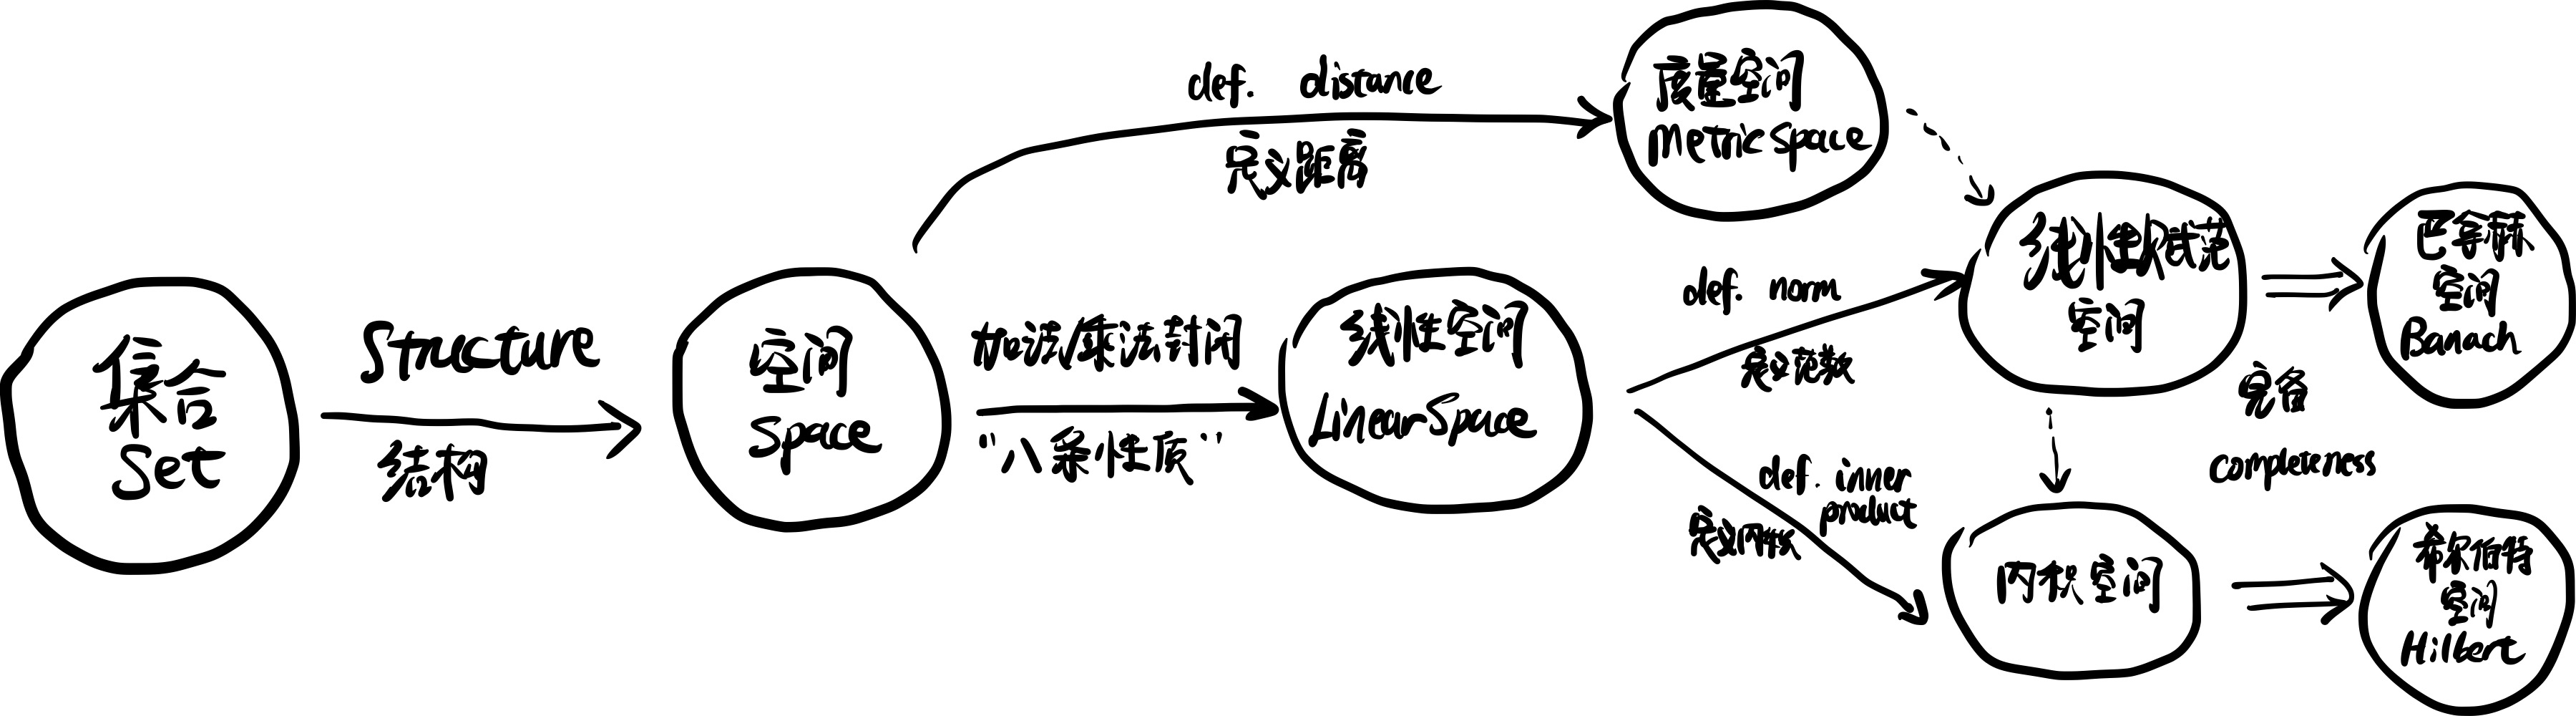
\includegraphics{C:/Users/Administrator/Documents/github/arxive/math/image-20231218171032793.png}
\caption{image-20231218171032793}
\end{figure}

\begin{newquote}
图改自知乎 @ 无尘粉笔, 本篇内容也 adapted from 他的这篇文章
\href{https://zhuanlan.zhihu.com/p/541226732}{什么是数学中的各种空间:线性空间、度量空间、赋范空间、内积空间、欧几里得空间、希尔伯特空间、巴拿赫空间?}
\end{newquote}

\subsubsection{附录:
行列式和递归}

考虑一个 \[n\times n\] 的行列式, 在计算时, 我们可以利用递归的思路:

\[n\times n\] 可以 reduce 成 \[n\] 个 \[(n-1)\times(n-1)\] 的行列式:
先把第一行第一列的元 \[a_{11}\] 拎出来,
然后计算去掉了第一行第一列的行列式, 并乘上 \[a_{11}\]; 然后把 \[a_{12}\]
拎出来, 计算去掉了第一行第二列的行列式; \ldots; 直到把 \[a_{1n}\]
拎出来, 执行类似的操作.

然后 \[(n-1)\times(n-1)\] 的行列式怎么计算呢? 出现了, 递归大法好!
我们可以将一个 \[(n-1)\times(n-1)\] 的行列式 reduce 成 \[(n-1)\] 个
\[(n-2)\times(n-2)\] 的行列式.

\ldots{}

不断重复上述操作, 直到 reduce 成许多个 \[2\times2\] 或者是 \[3\times3\]
的矩阵, 就可以用【026】提到的,
【左上向右下的对角线之和】减去【右上向左下的对角线之和】来计算了.

虽然听起来很繁琐, 但是计算大的行列式时, 这样大量重复,
但本身不复杂的运算, GPU (显卡) 最擅长了, 直接丢给计算机就可以了.
递归这种``套娃''的思路在编程中经常出现,
它和【007】中提到的归纳法其实也有一定的联系.
